\documentclass[aspectratio=169]{beamer}
\usetheme{Madrid}
\usecolortheme{default}
\usepackage[T1]{fontenc}
\usepackage[utf8]{inputenc}
\usepackage{graphicx}
\usepackage{booktabs}
\usepackage{hyperref}

\title{Air Quality Intelligence System}
\subtitle{Advanced Data Warehouse Technologies}
\author{Péter Dobosi (MW79ON)}
\institute{University of Pannonia}
\date{2025/26 Spring}

\begin{document}

% ----------------------------------------------------------
\begin{frame}
\titlepage
\end{frame}

% ----------------------------------------------------------
\begin{frame}{Problem Statement}
\begin{itemize}
  \item Air quality data is voluminous and time-series in nature
  \item Raw API data is unstructured (JSON) and unsuitable for analytics
  \item Need: a well-modeled analytical warehouse with ETL, SCD, ML predictions, and dashboards
\end{itemize}
\vspace{1em}
\textbf{Goal:} Build an end-to-end data warehouse pipeline from ingestion through
prediction to interactive analytical dashboards.
\note{~1 min --- motivate the DW approach.}
\end{frame}

% ----------------------------------------------------------
\begin{frame}{Architecture \& Data Flow}
\begin{figure}
\centering
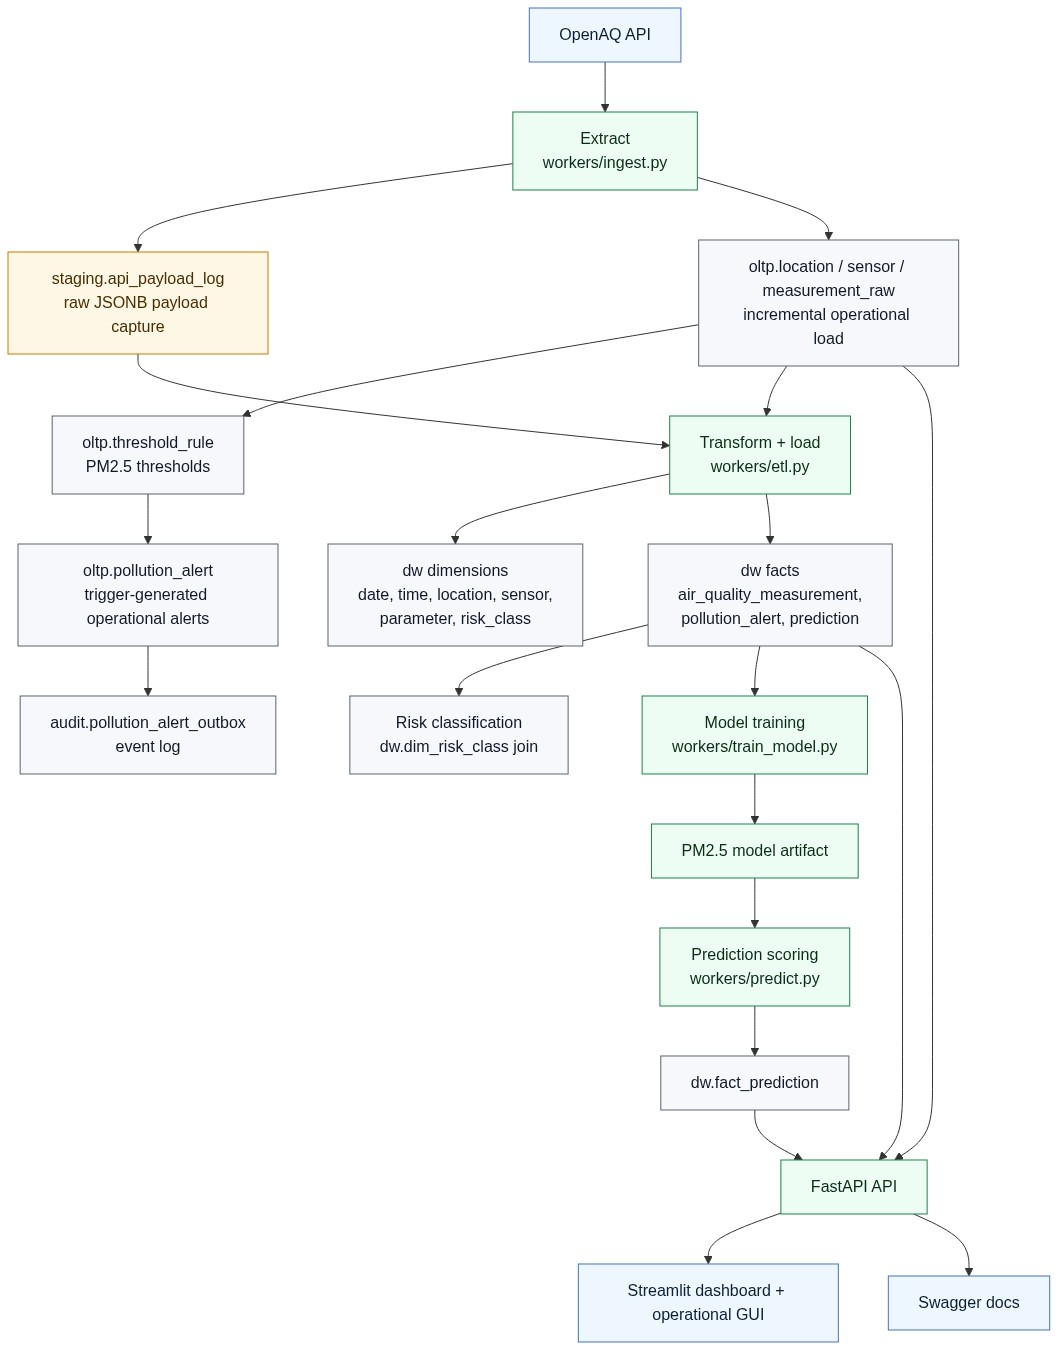
\includegraphics[width=0.65\textwidth,height=0.78\textheight,keepaspectratio]{../../diagrams/data_flow.png}
\end{figure}
\note{~1 min --- trace the flow: OpenAQ → staging → OLTP → ETL → DW → dashboard.}
\end{frame}

% ----------------------------------------------------------
\begin{frame}{Star Schema Design (Fact Constellation)}
\begin{figure}
\centering
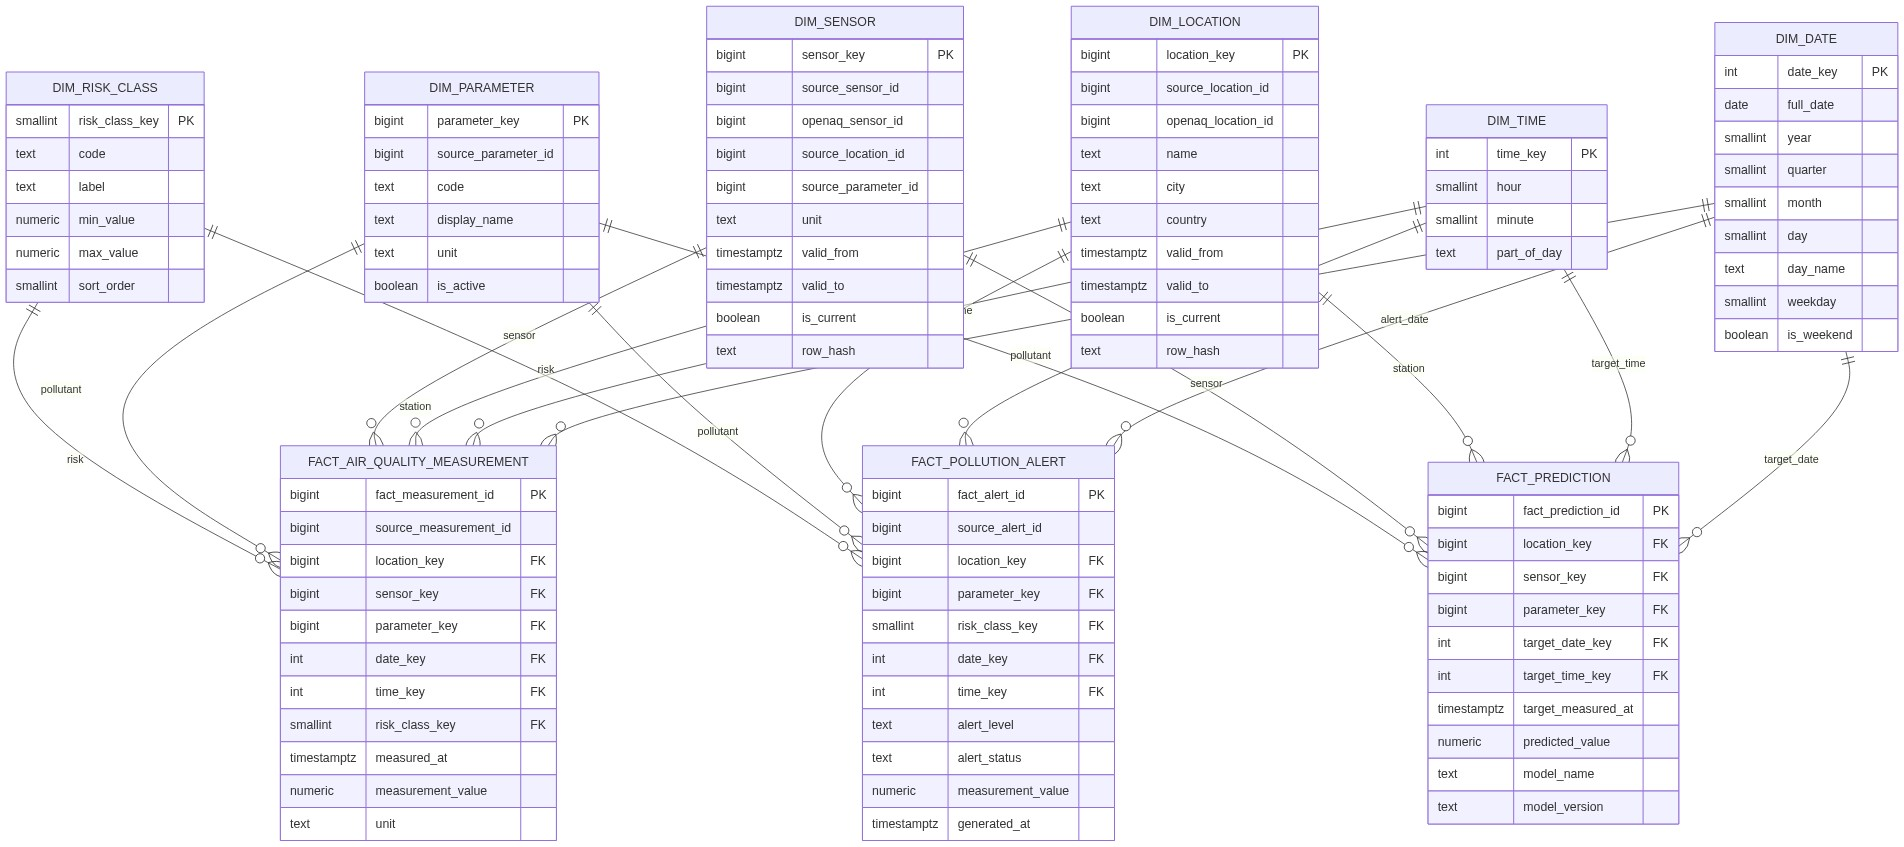
\includegraphics[width=0.62\textwidth,height=0.75\textheight,keepaspectratio]{../../diagrams/dw_star_schema.png}
\end{figure}
\vspace{-0.5em}
\small Three fact tables sharing conformed dimensions (galaxy schema pattern).
\note{~1.5 min --- explain facts vs dimensions, grain of each fact table.}
\end{frame}

% ----------------------------------------------------------
\begin{frame}{ETL Pipeline \& SCD Type~2}
\begin{itemize}
  \item Python ETL script: extract from OLTP → transform → load into DW
  \item Watermark-based incremental extraction (only new rows)
  \item \textbf{SCD Type~2} on \texttt{dim\_location} and \texttt{dim\_sensor}:
  \begin{itemize}
    \item Hash-based change detection (\texttt{row\_hash})
    \item Expire old row (\texttt{valid\_to}, \texttt{is\_current = false})
    \item Insert new version (\texttt{valid\_from = now()})
  \end{itemize}
  \item Conformed date/time dimensions pre-populated
\end{itemize}
\note{~1.5 min --- show ETL code structure, explain SCD2 flow.}
\end{frame}

% ----------------------------------------------------------
\begin{frame}{Demo: Air Quality Overview Dashboard}
\begin{itemize}
  \item KPIs: latest value, weekly average, station count, open alerts
  \item Trend chart with daily aggregation (avoids spaghetti)
  \item Worst station metric + latest-by-station table
  \item Sidebar filters: city, station, pollutant, date range
\end{itemize}
\vspace{0.5em}
\textit{Live demo: \url{https://mw79on-demo.online} → Air Quality Overview}
\note{~1.5 min --- show filters and chart updating.}
\end{frame}

% ----------------------------------------------------------
\begin{frame}{Demo: High-Risk Periods}
\begin{itemize}
  \item Alert heatmap: weekday × hour concentration
  \item Severity mix bar chart
  \item Alerts by pollutant and by station (top 10)
  \item Recent high-risk alert table
\end{itemize}
\vspace{0.5em}
\textit{Live demo: → High-Risk Periods page}
\note{~1 min --- highlight the heatmap pattern.}
\end{frame}

% ----------------------------------------------------------
\begin{frame}{Demo: Prediction Insights}
\begin{itemize}
  \item Random Forest model trained on DW historical data
  \item Features: hour, weekday, month, recent averages, location
  \item Chart: actual vs.\ predicted PM2.5 concentration
  \item Metrics: MAE \(\approx\) 0.91, RMSE \(\approx\) 1.21, R² \(\approx\) 0.73
  \item Predictions stored as \texttt{fact\_prediction} in the DW
\end{itemize}
\vspace{0.5em}
\textit{Live demo: → Prediction Insights page}
\note{~1.5 min --- show actual/predicted chart, point out error.}
\end{frame}

% ----------------------------------------------------------
\begin{frame}{Automated Refresh \& Scheduling}
\begin{itemize}
  \item Orchestration script: \texttt{scripts/run\_pipeline.sh}
  \item Modes: \texttt{full}, \texttt{ingest-etl}, \texttt{predict-only}, \texttt{train-predict}
  \item Stage gating: failure in ingest → ETL skipped
  \item Cron: ingest-etl every 3 hours, predict daily
  \item Logs written to \texttt{logs/} with status JSON
\end{itemize}
\note{~1 min --- show crontab, explain modes.}
\end{frame}

% ----------------------------------------------------------
\begin{frame}{Deployment}
\begin{columns}[T]
\begin{column}{0.55\textwidth}
\begin{itemize}
  \item Hetzner Cloud VM
  \item Docker Compose (5 services)
  \item Caddy: automatic HTTPS
  \item GitHub Actions CI/CD
  \item Single \texttt{git push} → deployed
\end{itemize}
\end{column}
\begin{column}{0.45\textwidth}
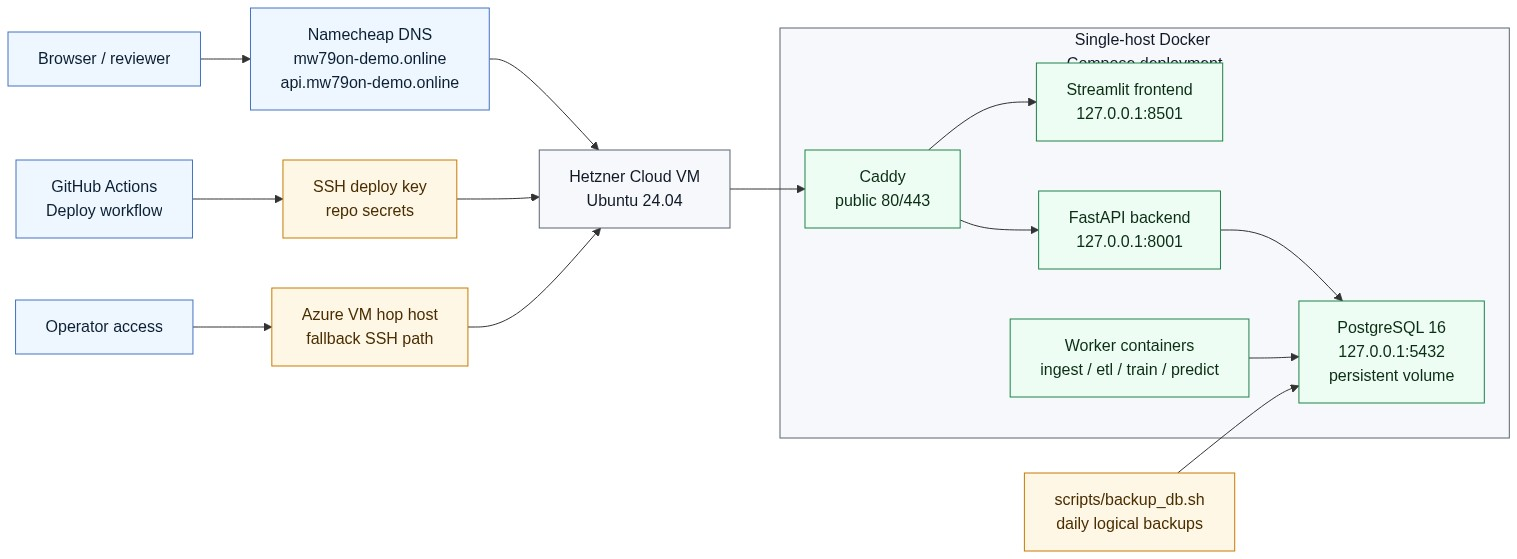
\includegraphics[width=\textwidth]{../../diagrams/deployment_architecture.png}
\end{column}
\end{columns}
\note{~1 min --- show GitHub Actions run, live URL.}
\end{frame}

% ----------------------------------------------------------
\begin{frame}{Summary \& Lessons Learned}
\begin{itemize}
  \item Star schema + SCD2 enables rich historical analytics
  \item Incremental ETL keeps the warehouse fresh without full rebuilds
  \item ML predictions as first-class DW facts enable comparison dashboards
  \item Daily aggregation solves multi-station chart readability
  \item Automated pipelines + CI/CD = hands-off operation
\end{itemize}
\vspace{1em}
\textbf{Live system:} \url{https://mw79on-demo.online}\\
\textbf{Source code:} \url{https://github.com/dobosipeter/advanced-data-warehouse-and-database-management-systems-submission}
\note{~1 min --- wrap up, invite questions.}
\end{frame}

\end{document}
